\newpage
\section{Chiến Lược Sao Lưu Dữ Liệu Với MinIO và AWS S3}

\subsection{Đặt Vấn Đề}

Trong hệ thống tích hợp dữ liệu, mỗi lần đồng bộ đều có khả năng ghi đè
hoặc biến đổi dữ liệu tại destination. Khi xảy ra các sự kiện bất thường —
lỗi pipeline, thay đổi schema không kiểm soát, hoặc dữ liệu nguồn bị hỏng —
cần có khả năng phục hồi về trạng thái trước đó một cách đáng tin cậy.
Yêu cầu này đặt ra bốn bài toán cụ thể:

\begin{enumerate}
    \item \textbf{Backup phòng ngừa:} Tạo snapshot trước mỗi lần sync để có
    điểm phục hồi ngay cả khi pipeline ghi dữ liệu sai.
    \item \textbf{Backup kiểm toán:} Lưu giữ vĩnh viễn snapshot tại thời điểm
    schema thay đổi — phục vụ truy vết lịch sử cấu trúc dữ liệu.
    \item \textbf{Backup định kỳ:} Đảm bảo luôn có bản sao dữ liệu hoàn chỉnh
    theo lịch, độc lập với hoạt động sync.
    \item \textbf{Lưu trữ vĩnh viễn trên cloud:} Nhân bản các backup quan trọng
    lên AWS S3 để đảm bảo tính bền vững và khả năng phục hồi ngay cả khi
    infrastructure nội bộ gặp sự cố.
\end{enumerate}

\subsection{Kiến Trúc Hai Tầng: MinIO và AWS S3}

Hệ thống sử dụng kiến trúc lưu trữ hai tầng:

\begin{itemize}
    \item \textbf{Tầng 1 — MinIO (primary):} Object storage self-hosted triển
    khai trên Docker, tương thích với giao thức Amazon S3. Mọi backup được ghi
    vào MinIO ngay lập tức. MinIO phục vụ cho các tác vụ restore và truy vấn
    thường xuyên nhờ độ trễ thấp trong môi trường nội bộ.
    \item \textbf{Tầng 2 — AWS S3 (secondary/permanent):} Dịch vụ object
    storage của Amazon Web Services, đóng vai trò kho lưu trữ vĩnh viễn. Admin
    có thể chủ động đẩy (sync) các file backup từ MinIO lên S3 để bảo toàn
    dữ liệu ngoài môi trường on-premise.
\end{itemize}

\begin{figure}[H]
\centering
\resizebox{\textwidth}{!}{%
\begin{tikzpicture}[
  trigger/.style={rectangle, draw, rounded corners,
                  minimum width=3.8cm, minimum height=0.75cm,
                  text centered, font=\small, fill=blue!8},
  svcbox/.style={rectangle, draw, rounded corners,
                  minimum width=3.2cm, minimum height=0.9cm,
                  text centered, font=\small, fill=orange!15},
  arrow/.style={->, >=stealth, thick},
  darrow/.style={->, >=stealth, thick, dashed}
]

%% --- Triggers (left) ---
\node[trigger] (presync) {Pre-sync Trigger};
\node[trigger, below=0.5cm of presync] (schema) {Schema Change Event};
\node[trigger, below=0.5cm of schema] (cron)
    {Scheduled (Ex: Sunday 2:00 AM)};
\node[trigger, below=0.5cm of cron] (manual)
    {Manual (POST /backup/trigger)};

%% --- BackupService (center) ---
\node[svcbox, right=3.5cm of schema, yshift=-0.65cm] (service) {BackupService};

%% --- MinIO ellipse (top right, small) ---
\node[ellipse, draw, fill=green!20,
      minimum width=2.2cm, minimum height=1.4cm,
      right=3.5cm of service, yshift=1.2cm]
    (minio) {MinIO (Primary)};

%% --- S3 ellipse (bottom right, small, clearly separated) ---
\node[ellipse, draw, fill=yellow!30,
      minimum width=2.4cm, minimum height=1.4cm,
      right=3.5cm of service, yshift=-1.2cm]
    (s3) {AWS S3 (Permanent)};

%% --- Triggers -> BackupService ---
\draw[arrow] (presync.east)  -| (service.north);
\draw[arrow] (schema.east)   -- (service.west);
\draw[arrow] (cron.east)     -| (service.south);
\draw[arrow] (manual.east)   -| (service.south);

%% --- BackupService -> MinIO ---
\draw[arrow] (service.east) -- node[above, font=\footnotesize]{auto}
    (minio.west);

%% --- BackupService -> S3 ---
\draw[arrow] (service.east) -- node[below, font=\footnotesize]{on-demand}
    (s3.west);

%% --- Sync arrow MinIO -> S3 ---
\draw[darrow] (minio.south) -- node[right, font=\footnotesize]{sync}
    (s3.north);

\end{tikzpicture}
}%
\caption{Kiến trúc lưu trữ hai tầng: MinIO và AWS S3}
\label{fig:backup-arch}
\end{figure}


\subsubsection{Cấu Hình Triển Khai}

MinIO được tích hợp vào \texttt{docker-compose.yml} cùng với phần còn lại của
hệ thống:

\begin{lstlisting}[language=python, caption={Cấu hình MinIO trong docker-compose.yml}]
services:
  minio:
    image: minio/minio:latest
    container_name: data-hub-minio
    command: server /data --console-address ":9001"
    ports:
      - "9000:9000"   # S3 API endpoint
      - "9001:9001"   # Web Console
    environment:
      MINIO_ROOT_USER: ${MINIO_ACCESS_KEY}
      MINIO_ROOT_PASSWORD: ${MINIO_SECRET_KEY}
    volumes:
      - minio_data:/data
    restart: always
\end{lstlisting}

Cấu hình AWS S3 được truyền vào backend qua biến môi trường:

\begin{lstlisting}[language=bash, caption={Biến môi trường AWS S3}]
AWS_ACCESS_KEY_ID=<access-key>
AWS_SECRET_ACCESS_KEY=<secret-key>
AWS_REGION=ap-southeast-2
AWS_S3_BUCKET=data-integration-hub-bucket
\end{lstlisting}

\subsection{Bốn Loại Trigger Backup}

\subsubsection{Trigger 1: Pre-Sync Backup}

Đây là lớp bảo vệ quan trọng nhất. Ngay trước khi \texttt{syncOneTable()}
bắt đầu ghi dữ liệu vào PostgreSQL, một snapshot đầy đủ của bảng được tạo
và lưu lên MinIO:

\begin{lstlisting}[caption={Pre-sync backup trong syncOneTable()}]
await this.backupService.backupTable(schema.tableName, 'pre-sync');
// Sau do moi bat dau fetch va sync
\end{lstlisting}

Chỉ những bảng có \texttt{status = 'stable'} mới đến được bước
\texttt{syncOneTable()} — pipeline lọc bảng không ổn định trước khi vào vòng
lặp sync.

\subsubsection{Trigger 2: Schema Change Backup}

Khi \texttt{SchemaRegistryService} phát hiện một bảng thay đổi cấu trúc,
hệ thống emit event \texttt{schema.changed}. \texttt{BackupService} lắng nghe
event này và tạo snapshot ngay lập tức — trước khi bảng bị đánh dấu
\texttt{changed} và khóa khỏi chu kỳ sync tiếp theo:

\begin{lstlisting}[caption={Xử lý event schema.changed}]
@OnEvent('schema.changed')
async handleSchemaChanged(payload: { tableName: string }) {
  await this.backupTable(payload.tableName, 'schema-change');
}
\end{lstlisting}

Đây là snapshot cuối cùng của dữ liệu tương thích với schema cũ, có giá trị
kiểm toán cao và được giữ vĩnh viễn.

\subsubsection{Trigger 3: Scheduled Weekly Backup}

Mỗi Chủ nhật lúc 2:00 AM, hệ thống tự động backup toàn bộ bảng
\texttt{stable} và thực hiện cleanup các file quá hạn:

\begin{lstlisting}[caption={Scheduled backup mỗi Chủ nhật 2:00 AM}]
@Cron('0 2 * * 0')
async handleWeeklyBackup() {
  await this.backupAllStable('scheduled');
  await this.cleanupOldBackups();
}
\end{lstlisting}

\subsubsection{Trigger 4: Manual Backup}

Admin có thể kích hoạt backup bất kỳ lúc nào qua API
\texttt{POST /backup/trigger}, chỉ định một hoặc nhiều bảng cụ thể, hoặc bỏ
trống để backup toàn bộ bảng stable.

\subsection{Cấu Trúc Lưu Trữ Trong MinIO}


Tất cả backup được tổ chức trong bucket \texttt{data-hub-backups} theo cấu
trúc phân cấp thống nhất:

\begin{center}
\texttt{\{trigger\}/\{tableName\}/\{ISO-timestamp\}.json}
\end{center}

\begin{lstlisting}[caption={Cấu trúc thư mục trong bucket MinIO}]
data-hub-backups/
|-- pre-sync/
|   |-- nguoi_hoc/
|   |   |-- 2026-04-20T08-30-00-000Z.json
|   |   `-- 2026-04-21T09-15-22-451Z.json
|   `-- nh_dao_tao/
|       `-- 2026-04-21T09-15-25-112Z.json
|
|-- schema-change/
|   `-- nguoi_hoc/
|       |-- 2026-03-15T14-22-10-334Z.json
|       `-- 2026-04-10T09-05-44-218Z.json
|
|-- scheduled/
|   `-- nguoi_hoc/
|       |-- 2026-04-13T02-00-05-000Z.json
|       `-- 2026-04-20T02-00-03-000Z.json
|
`-- manual/
    `-- nguoi_hoc/
        `-- 2026-04-20T15-00-00-000Z.json
\end{lstlisting}

\begin{figure}
    \centering
    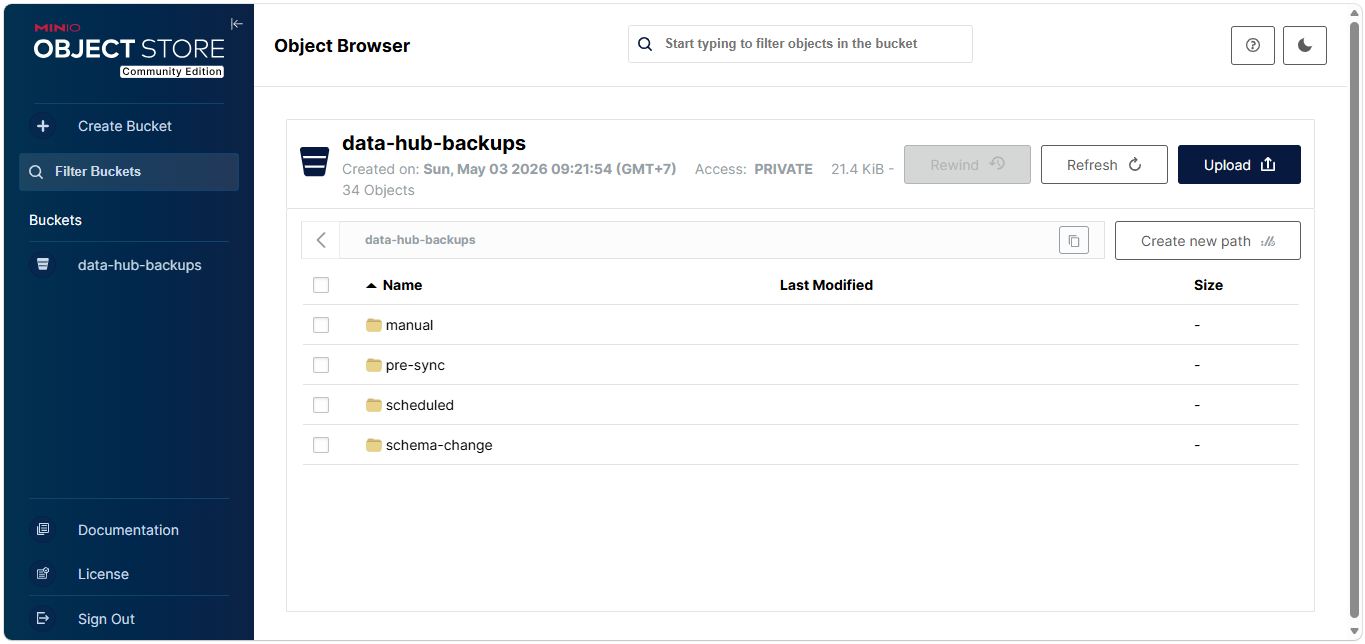
\includegraphics[width=1\linewidth]{graphics/MINIO_main.png}
    \caption{Giao diện cấu trúc trong MINIO}
    \label{fig:dashboard-ui}
\end{figure}

\begin{figure}
    \centering
    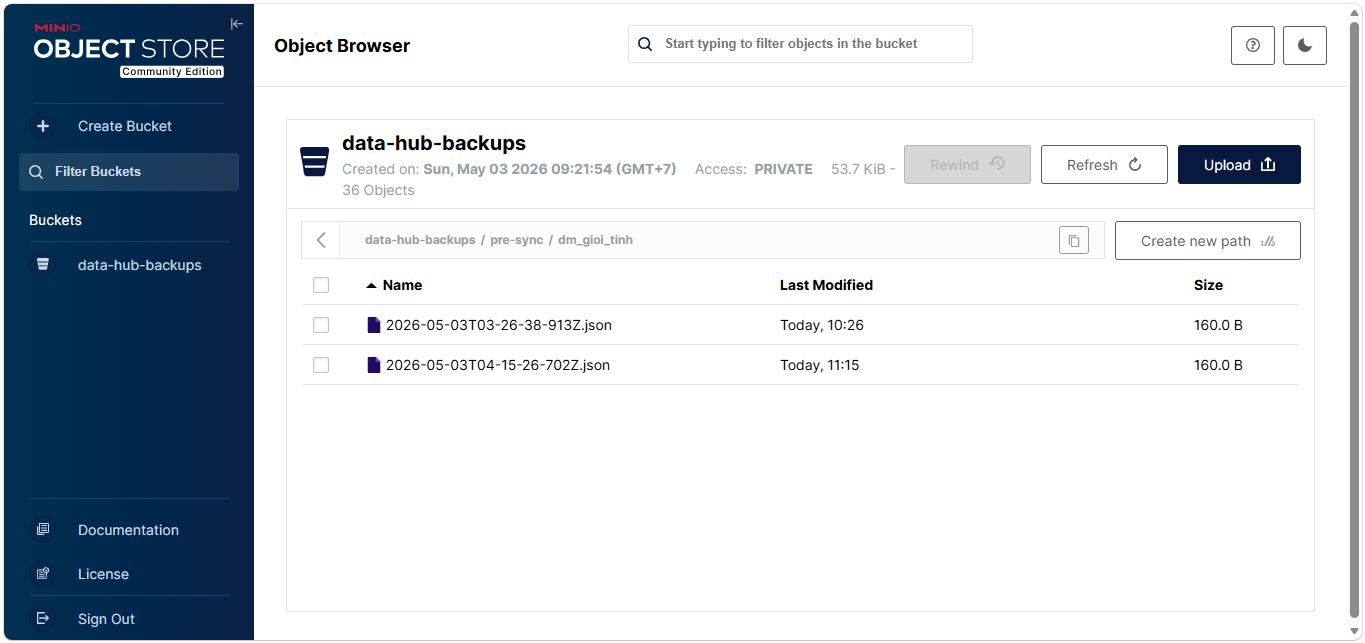
\includegraphics[width=1\linewidth]{graphics/MINIO_path.png}
    \caption{Các file Backup cho một bảng trong MINIO}
    \label{fig:dashboard-ui}
\end{figure}


Mỗi file backup là một JSON object gồm phần \texttt{meta} và \texttt{data}:

\begin{lstlisting}[caption={Cấu trúc file backup JSON}]
{
  "meta": {
    "tableName": "nguoi_hoc",
    "trigger": "pre-sync",
    "backedUpAt": "2026-04-21T02:15:30.000Z",
    "recordCount": 68411
  },
  "data": [
    { "id": 1, "ho": "Nguyen Van", "ten": "A", ... }
  ]
}
\end{lstlisting}

JSON được chọn thay vì CSV vì giữ nguyên kiểu dữ liệu (\texttt{DateTime},
\texttt{Boolean}, \texttt{null}) và tương thích trực tiếp với Prisma
\texttt{createMany()} khi restore.

\subsection{Chính Sách Lưu Giữ (Retention Policy)}

\begin{table}[H]
\centering
\caption{Chính sách lưu giữ backup theo loại trigger}
\label{tab:retention}
\renewcommand{\arraystretch}{1.4}
\begin{tabular}{|l|c|p{7.5cm}|}
\hline
\textbf{Loại trigger} & \textbf{Thời gian giữ} & \textbf{Lý do} \\
\hline
\texttt{pre-sync} & 30 ngày
    & Đủ để phát hiện và rollback lỗi sync trong chu kỳ vận hành. \\
\hline
\texttt{scheduled} & 60 ngày
    & Lưu ~8 bản weekly — đủ truy vết biến động 2 tháng gần nhất. \\
\hline
\texttt{schema-change} & Vĩnh viễn
    & Audit trail lịch sử thay đổi cấu trúc dữ liệu. \\
\hline
\texttt{manual} & 30 ngày
    & Backup thủ công thường phục vụ mục đích ngắn hạn. \\
\hline
\end{tabular}
\end{table}

Cleanup được thực thi tự động sau mỗi weekly backup và có thể gọi thủ công
qua \texttt{POST /backup/cleanup}.

\subsection{Cơ Chế Đồng Bộ Lên AWS S3}

\subsubsection{Mục Tiêu}

MinIO là storage nội bộ chạy trên cùng máy chủ với hệ thống. Trong trường hợp
máy chủ gặp sự cố nghiêm trọng (mất điện, hỏng ổ đĩa), toàn bộ dữ liệu
MinIO có thể bị mất cùng lúc. AWS S3 đóng vai trò lớp lưu trữ thứ hai —
địa lý phân tán, độ bền \textbf{99.999999999\%} (11 số 9) theo cam kết SLA
của Amazon.


\begin{figure}[H]
    \centering
    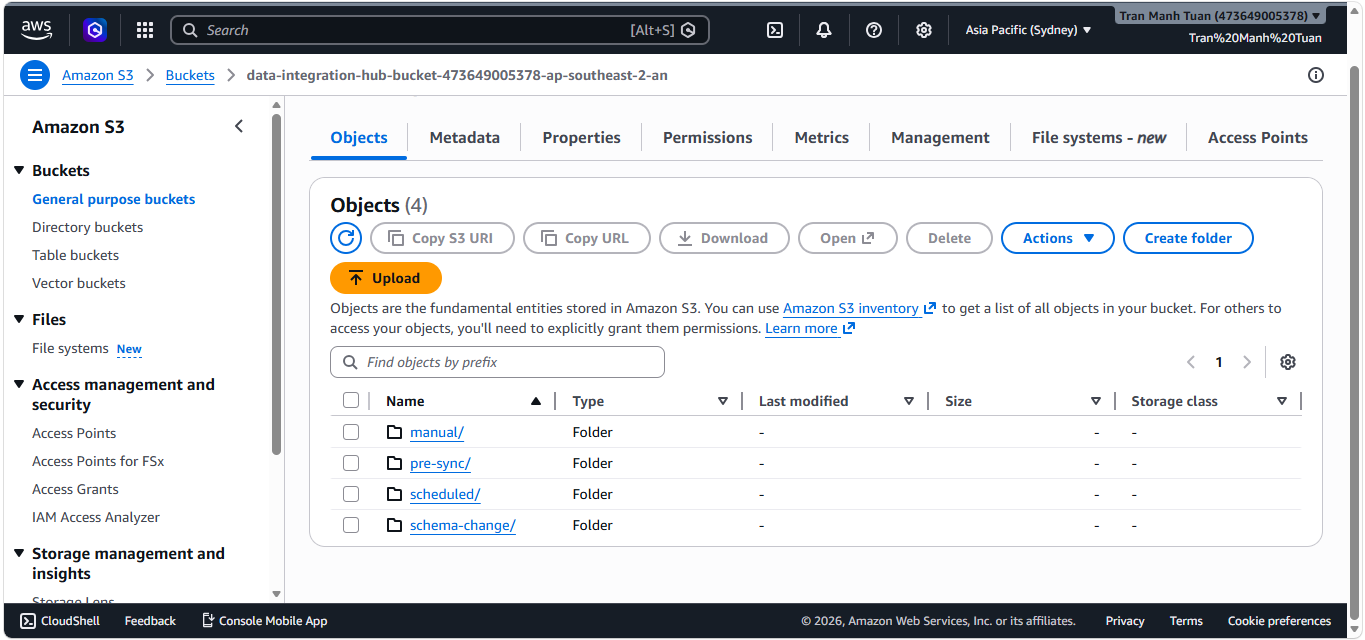
\includegraphics[width=1\linewidth]{graphics/S3.png}
    \caption{Giao diện lưu trữ file trên S3 }
    \label{fig:dashboard-ui}
\end{figure}

\subsubsection{Luồng Hoạt Động}

Đồng bộ lên S3 được thiết kế theo mô hình \textbf{on-demand} (theo yêu cầu)
thay vì tự động sau mỗi backup, nhằm tránh tạo ra bottleneck I/O trong các
chu kỳ sync tần suất cao:

\begin{enumerate}
    \item Admin gọi API sync (một file hoặc toàn bộ).
    \item \texttt{S3Service} kiểm tra file đã tồn tại trên S3 chưa bằng
    \texttt{HeadObjectCommand}.
    \item Nếu chưa có: tải file JSON từ MinIO về bộ nhớ, upload lên S3 bằng
    \texttt{PutObjectCommand}.
    \item Nếu đã có: bỏ qua — tránh upload trùng lặp không cần thiết.
\end{enumerate}

\subsubsection{Trạng Thái Đồng Bộ}

API \texttt{GET /backup/list} trả về thêm trường \texttt{s3Status} cho mỗi
file backup, phản ánh tình trạng đồng bộ giữa MinIO và S3:

\begin{table}[H]
\centering
\caption{Các giá trị trạng thái đồng bộ S3}
\label{tab:s3-status}
\renewcommand{\arraystretch}{1.4}
\begin{tabular}{|l|p{9cm}|}
\hline
\textbf{Giá trị} & \textbf{Ý nghĩa} \\
\hline
\texttt{not\_synced}
    & File chỉ tồn tại trên MinIO, chưa được upload lên S3. \\
\hline
\texttt{synced}
    & File đã được upload lên S3 và \texttt{lastModified} trên MinIO
      $\leq$ \texttt{LastModified} trên S3 — hai phiên bản đồng nhất. \\
\hline
\texttt{out\_of\_date}
    & File tồn tại trên S3 nhưng phiên bản trên MinIO mới hơn —
      cần sync lại. \\
\hline
\end{tabular}
\end{table}

Trạng thái được tính bằng cách so sánh \texttt{lastModified} của từng object:
nếu thời điểm chỉnh sửa trên MinIO $\leq$ thời điểm upload lên S3 thì
file được coi là \texttt{synced}; ngược lại là \texttt{out\_of\_date}.
Để tránh gọi \texttt{HeadObject} cho từng file (chi phí $O(n)$ request),
hệ thống sử dụng \texttt{ListObjectsV2} một lần duy nhất để lấy toàn bộ
danh sách S3 và xây dựng \texttt{Map<key, LastModified>} trước khi đối chiếu.

\subsubsection{Fire-and-Forget cho Sync Hàng Loạt}

Khi sync toàn bộ bucket (có thể lên đến hàng trăm file), tác vụ mất nhiều
phút để hoàn thành. Nếu xử lý đồng bộ (\textit{blocking}), HTTP client hoặc
API Gateway sẽ timeout trước khi nhận được response.

Hệ thống giải quyết bằng mô hình \textbf{fire-and-forget}: endpoint trả về
response \texttt{200} ngay lập tức, trong khi tác vụ sync tiếp tục chạy nền:

\begin{lstlisting}[caption={Fire-and-forget cho sync-s3/all}]
@Post('sync-s3/all')
syncAllToS3() {
  // Khong await - tra response ngay, sync chay nen
  this.backupService.syncAllToS3().catch(() => {});
  return {
    message: 'S3 sync dang chay nen. Kiem tra log de xem tien trinh.'
  };
}
\end{lstlisting}

\subsection{API Quản Lý Backup}

\begin{table}[H]
\centering
\caption{Các endpoint quản lý backup}
\label{tab:backup-api}
\renewcommand{\arraystretch}{1.4}
\begin{tabular}{|l|l|p{5.5cm}|}
\hline
\textbf{Method} & \textbf{Endpoint} & \textbf{Mô tả} \\
\hline
\texttt{POST} & \texttt{/backup/trigger}
    & Backup thủ công một hoặc nhiều bảng. \\
\hline
\texttt{GET} & \texttt{/backup/list?prefix=...}
    & Liệt kê file backup kèm \texttt{s3Status}. \\
\hline
\texttt{POST} & \texttt{/backup/download}
    & Trả về presigned URL (1 giờ) để tải file từ MinIO. \\
\hline
\texttt{DELETE} & \texttt{/backup/file}
    & Xóa một file backup khỏi MinIO. \\
\hline
\texttt{POST} & \texttt{/backup/restore}
    & Restore một bảng từ file backup về PostgreSQL. \\
\hline
\texttt{POST} & \texttt{/backup/cleanup}
    & Xóa các file backup quá hạn theo retention policy. \\
\hline
\texttt{POST} & \texttt{/backup/sync-s3}
    & Đồng bộ một file cụ thể từ MinIO lên S3. \\
\hline
\texttt{POST} & \texttt{/backup/sync-s3/all}
    & Đồng bộ toàn bộ bucket lên S3 (chạy nền). \\
\hline
\end{tabular}
\end{table}

\subsection{Cơ Chế Restore}

Khi cần phục hồi dữ liệu, hệ thống thực hiện theo chiến lược
\textbf{overwrite}: xóa toàn bộ bảng rồi chèn lại từ file backup.
Trước khi restore, hệ thống tự động tạo thêm một snapshot \texttt{manual}
của trạng thái hiện tại — đây là lớp bảo vệ phòng trường hợp admin restore
nhầm file.

Do bảng \texttt{nguoi\_hoc} có hơn 68.000 bản ghi, việc insert toàn bộ trong
một transaction sẽ vượt quá timeout 5.000 ms của Prisma interactive
transaction. Hệ thống giải quyết bằng cách chia nhỏ thành các batch 1.000
bản ghi và insert tuần tự bên ngoài transaction:

\begin{lstlisting}[caption={Batch INSERT khi restore}]
const BATCH_SIZE = 1000;
for (let i = 0; i < data.length; i += BATCH_SIZE) {
  const batch = data.slice(i, i + BATCH_SIZE);
  await this.prisma[modelName].createMany({
    data: batch,
    skipDuplicates: true
  });
}
\end{lstlisting}

\subsection{Đánh Giá}

\subsubsection{Ưu Điểm}

\begin{itemize}
    \item \textbf{Bảo vệ nhiều lớp:} Ba trigger tự động đảm bảo luôn có điểm
    phục hồi gần nhất bất kể nguyên nhân sự cố.
    \item \textbf{Lưu trữ địa lý phân tán:} Kết hợp MinIO nội bộ và AWS S3
    đám mây — sự cố tại một nơi không ảnh hưởng đến phiên bản còn lại.
    \item \textbf{Audit trail đầy đủ:} Backup \texttt{schema-change} lưu vĩnh
    viễn cho phép tái hiện lịch sử dữ liệu theo từng mốc thay đổi cấu trúc.
    \item \textbf{Khả năng quan sát:} Trường \texttt{s3Status} trong API list
    cho phép admin theo dõi tình trạng đồng bộ của từng file mà không cần
    truy cập trực tiếp vào AWS Console.
\end{itemize}

\subsubsection{Hạn Chế và Hướng Phát Triển}

Phương án hiện tại thực hiện \texttt{SELECT *} toàn bộ bảng trước mỗi lần
sync. Với bảng \texttt{nguoi\_hoc} có 68.411 bản ghi, mỗi file backup có
kích thước khoảng 50--80 MB. Hai hướng cải tiến được đề xuất: (1) sử dụng
\textit{incremental backup} — chỉ lưu delta so với lần trước; (2) nén bằng
\texttt{gzip} trước khi upload để giảm dung lượng khoảng 60--70\%.

Cơ chế đồng bộ S3 hiện hoạt động theo mô hình on-demand. Hướng phát triển
tiếp theo là tự động hóa: sau mỗi lần backup thành công, hệ thống tự đẩy
file mới lên S3 mà không cần admin can thiệp thủ công.
